\documentclass[oneside, a5paper,10pt]{article}

%------------Служебная информация, не меняй----------
\usepackage[TS1,T2A]{fontenc}
\usepackage[utf8]{inputenc}
\usepackage[english,russian]{babel}
\usepackage{indentfirst} %отступ в начале параграфа
\usepackage{amsmath,amsthm,amssymb} %математические библиотеки
\usepackage{graphicx}%Вставка картинок правильная
\usepackage{float}%"Плавающие" картинки
\usepackage{wrapfig}%Обтекание фигур (таблиц, картинок и прочего)
\usepackage{fancyhdr} %Колонтитул
\usepackage{geometry}
\geometry{
    left=1.5cm,% 1.9
    top=1.5cm,% 1.5 
    right=1.5cm,% 1.9
    bottom=1.5cm,% 1.5
    headsep=0.5cm,%
    footskip=0.5cm,%
    includehead,%
    includefoot}
\textwidth 110mm
\textheight 170mm
\linespread{1.0}
\setlength{\parskip}{3pt}
%-----------------------------------------------------

\begin{document}
%--------Колонтитул конференции - не менять------------
    \pagestyle{fancy}
    \fancyhead{}\fancyfoot{}
    \fancyhead[C]{Мультидисциплинарная молодежная конференция Центрального университета «Научный телеграф»}
    \cfoot{\thepage}
%------------------------------------------------------

%--------Название статьи, лишнюю строку удали----------
    \centerline{\bf СРАВНЕНИЕ МЕТОДОВ КЛАССИФИКАЦИИ ВЕБ-КОНТЕНТА} %название статьи
    \centerline{\bf ПО URL И ЗАГОЛОВКАМ СТРАНИЦ} %удали лишнее

    \smallskip %отступ
%--------Информация об авторах -----------------------
    \centerline{\bf}
    \centerline{\bf \ \ И. А. Дулина $^{1,*}$,   \ \ П.~А. Мартынюк $^{1}$}
    \smallskip
    \centerline{$^{1}$ МГТУ им. Н.Э. Баумана}
    \centerline{$^{*}$\it email: irisdulina@yandex.ru}
%-------------------------------------------------------
    \bigskip %отступ

%--------Аннотация в 3 предложения-----------------------

    В работе сравниваются методы классификации веб-ресурсов на зашумлённом несбалансированном датасете. Рассмотрены TF-IDF с логистической регрессией, FastText и мультиязычная модель семейства BERT. FastText показывает наилучший F1-score (0.988) при минимальных вычислительных затратах.

    \medskip
    \textit{Ключевые слова:} классификация текста, TF-IDF,
    FastText, BERT, фильтрация веб-контента, зашумлённые данные.
    \medskip

    \noindent\textbf{Введение.}
    Фильтрация нежелательного веб-контента востребована в системах родительского контроля и корпоративных сетях. В высоконагруженных системах анализ полного текста нецелесообразен, поэтому задача сводится к классификации по URL и заголовку. Цель работы – сравнение методов с точки зрения качества и вычислительной эффективности.

    \noindent\textbf{Данные и методология.}
    Датасет~\cite{dataset} (135 309 записей) имеет дисбаланс 7:1 и шум разметки.
    Предобработка включает извлечение значимых частей домена и
    токенизацию заголовков с фильтрацией стоп-слов. Сравниваются подходы к векторизации и классификации: TF-IDF + LogReg; FastText~\cite{Joulin} с символьными
    n-граммами; компактный трансформер Multilingual-MiniLM~\cite{Wang20}. Cреда Google Colab: GPU NVIDIA T4, CPU Intel Xeon (2.20 ГГц). Инференс TF-IDF и FastText – на CPU, BERT – на GPU, что ограничивает его применение.

    \noindent\textbf{Результаты.} Результаты представлены в таблице~\ref{Tabl1}. FastText превосходит BERT по F1 и скорости. При этом BERT чаще допускает ложноположительные ошибки, что предпочтительно для задач фильтрации (рис.~\ref{Comparison}).
    \begin{table}[h]
        \caption{\label{Tabl1} Сравнение моделей
            (инференс на 5000 примеров)}
        \begin{center}
            \begin{tabular}{|l|c|c|c|}
                \hline
                \textbf{Модель} & \textbf{F1} &
                \textbf{Время, с} & \textbf{RAM, МБ} \\ \hline
                TF-IDF + LR   & 0.972           & $\sim$0.002 & $\sim$29   \\ \hline
                FastText      & \textbf{0.9877} & $\sim$0.13  & $\sim$93   \\ \hline
                MiniLM (BERT) & 0.9853          & $\sim$309   & $\sim$1460 \\ \hline
            \end{tabular}
        \end{center}
    \end{table}

    Анализ ошибок показал: 190 общих ошибок, вызванных шумом разметки; TF-IDF имеет 761 уникальную ошибку из-за слабого учета морфем; FastText и BERT взаимодополняют друг друга (105 и 100 уникальных верных предсказаний): их расхождения часто связаны с дефектами разметки датасета, а не ошибками моделей. UMAP-визуализация подтверждает хорошее разделение классов (рис.~\ref{Comparison}).

    \begin{figure}[!h]
        \center
        
\includegraphics[width=0.36\linewidth]{cm_fasttext.png}
        
\includegraphics[width=0.36\linewidth]{cm_bert.png}
        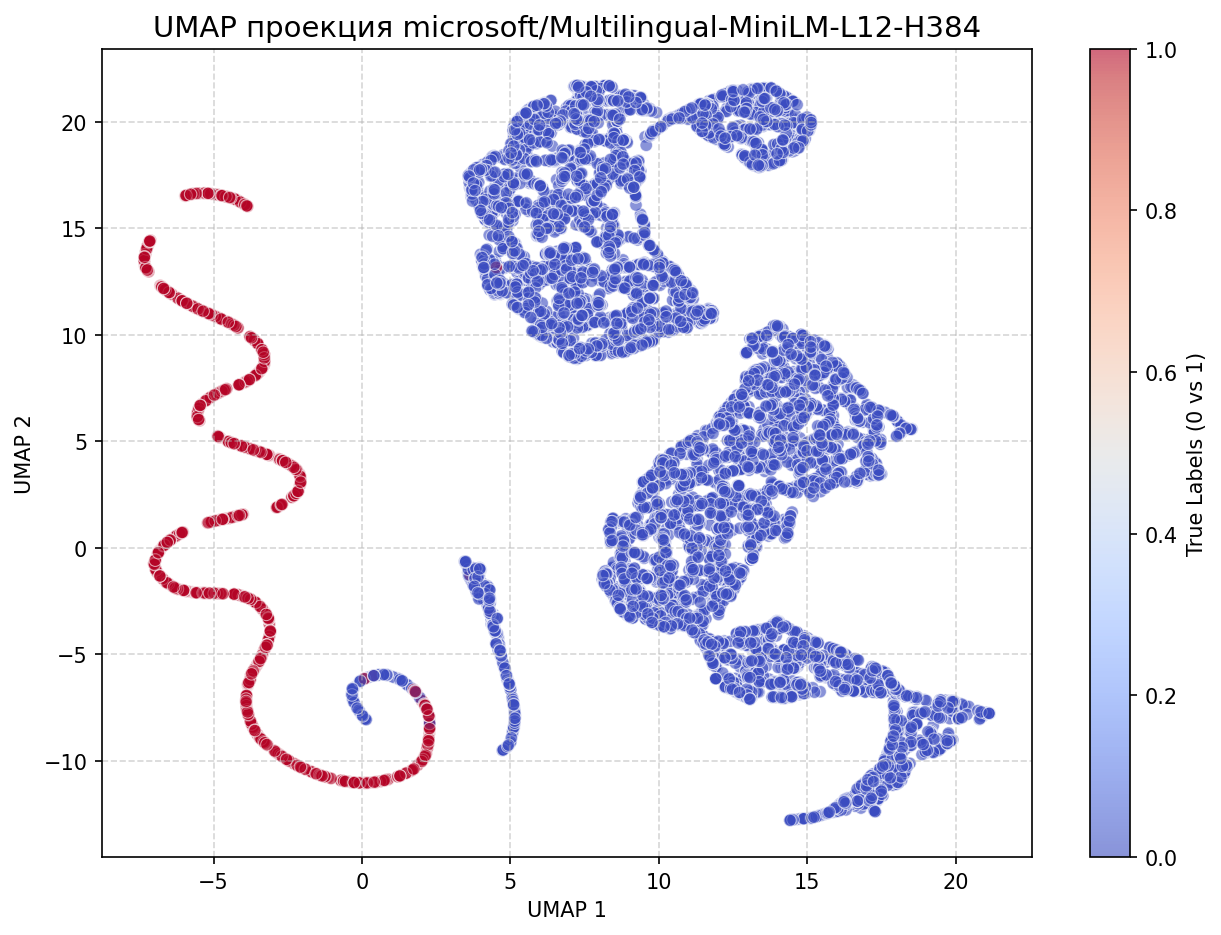
\includegraphics[width=0.26\linewidth]{bert_umap.png}
        \caption{Матрицы ошибок FastText и MiniLM (слева, центр) и UMAP-визуализация эмбеддингов MiniLM (справа):
        красный кластер – сайты для взрослых, синий – обычные}
        \label{Comparison}
    \end{figure}

    \noindent\textbf{Заключение.}
    Модель FastText обеспечивает лучшее соотношение качества и скорости. Модель BERT демонстрирует более предпочтительное распределение ошибок и устойчивость к сложным случаям. Перспективное
    направление – ансамблевый подход: FastText для
    потоковой фильтрации, BERT для валидации сложных случаев.

    \begin{thebibliography}{00}

        \setlength{\itemsep}{1.0pt plus 1.0pt}
        \bibitem{dataset}
        Датасет Porn Detection. Kaggle [Электронный ресурс]. ---
        URL: https://www.kaggle.com/datasets/mickleburg/ml-2026-spring-porn-detection
        (дата обращения: 17.04.2026).

        \bibitem{Joulin}
        Joulin A., Grave E., Bojanowski P., Mikolov T.
        Bag of Tricks for Efficient Text Classification //
        Proc. EACL. --- 2017. --- P. 427--431.

        \bibitem{Wang20}
        Wang W., Wei F., Dong L., Bao H., Yang N., Zhou M.
        MiniLM: Deep Self-Attention Distillation for
        Task-Agnostic Compression of Pre-Trained Transformers //
        Proc. NeurIPS. --- 2020.

    \end{thebibliography}

\end{document}

